\section{Background}
\par Traditional network defenses consist of largely static tools; firewalls and \acp{IDS} form the backbone of protection in most information technology shops.  Recently, however, there has been an interest in more active defense mechanisms, such as reputation and trust-based security \cite{Untrustworthiness} and \ac{NASR} \cite{APOD, NAH}. This paper focuses on the latter in a military setting.

\par At a high level, the concept of \ac{NASR} is simple: rather than a system sitting on a single \ac{IP} address, it changes its address rapidly, hopping amongst a set of \ac{IP} addresses assigned to it. This is similar in concept to a frequency hopping radio, although the effect is different. 

\par Normally an attacker wishing to target a given network gains a great deal of intelligence through simple scanning, checking each \ac{IP} inside the network and then checking each port on the active \acp{IP} to see what services are available. With this knowledge, the attacker may find entrance into the network. \ac{IP} hopping mitigates this issue by making it difficult to probe the network \cite{BBNDYNAT} and quickly invalidating any network map the attacker does manage to generate. Even if they locate a system's internal \ac{IP} address at some point in time, the address will change a few moments later.

\par Extensive research shows the utility of address-space randomization as a tool for obfuscating network traffic \cite{BBNDYNAT, NAH, TAO}. Further work demonstrates its usefulness as a tool for avoiding \ac{IP} hitlist-based attacks, wherein malware is given a preset list of \acp{IP} to attack \cite{NASR}. Finally, Sandia discusses virtually every aspect of this area \cite{SandiaDynat} and includes the assertion that \ac{IPsec} and \ac{DYNAT} could complement each other. In particular, Sandia suggests that \ac{DYNAT} allows networks to quickly drop invalid packets without performing expensive \ac{IPsec} operations.

%\par In this paper we propose an \ac{IP} address hopping system called the Address Routing Gateway (\ac{ARG}). It incorporates many of the features of previous address-hopping schemes, with an eye on the specific needs of the military. In this context each of the existing systems presents drawbacks that we attempt to avoid with \ac{ARG}. Additionally, the design of ARG is intended to allow its future integration with a traditional IDS and honeypot, potentially gaining additional insight into an attacker's behavior.

\par This suggestion by Sandia is the focus of this research. Section \ref{sec:problem_def} of this paper more closely defines the question being addressed. Section \ref{sec:boundaries} defines the \ac{SUT}, including limitations and scope. 

\section{Problem Definition}
\label{sec:problem_def}
\subsection{Goals and Hypothesis}
\label{sec:goals}
\par This research determines the validity of the Sandia claim \cite{SandiaDynat}: would a \ac{DYNAT} allow reliable packet filtering? This question is answered by measuring the accuracy of packet classification. If the claim is validated, it is safe to state that the introduction of \ac{DYNAT} into a network would positively benefit security.

%\par The software developed and tested here attempts to interfere minimally with the network, a critical requirement for the real-world deployment of such technology. Systems \ac{ARG} touches---both inside and outside the ``protected'' networks---do not need any modifications to continue to function. The research done here provides data on whether this is true as a side effect, potentially valuable information for an organization considering employing a \ac{DYNAT} solution. However, validation of this design goal is not a primary objective. 

\par The working hypothesis for this research is, as speculated by Sandia, a \ac{DYNAT} system allows for quick identification of unexpected (and potentially malicious) packets entering a network. There are few identifiers within the scope of \ac{DYNAT} by which outgoing packets could be filtered. Given that, no filtering is done for outbound packets and hence no change in behavior is observed when compared to the control network. 

\subsection{Approach}
\label{sec:approach}
% TBD too low-level?
\par This research is done on a test network with nodes representing the types of hosts found on a typical, corporate-style network. These include trusted hosts inside trusted networks which communicate freely, internal and external servers that must be accessible to hosts inside these trusted networks, and malicious hosts outside the networks. A configurable custom \ac{DYNAT} sits in front of the trusted networks. \tbd{diagram for last sentence}

\par Traffic generators and collectors run on this network, determining which traffic flows successfully make it to their destination. More importantly, they compare what should have been denied to what the \ac{DYNAT} actually denied. Measurements of allowed traffic flows between networks with a \ac{DYNAT} in place and without is used to answer the research question.

%\par If it is shown... then... QED

\FloatBarrier
\section{System Boundaries}
\label{sec:boundaries}
\par The \ac{SUT} is \ac{ARG}, a custom \ac{DYNAT} solution developed specifically for this effort. The basic components of this system, the various inputs into the system, possible outputs, and the metrics provided are illustrated in Figure \ref{fig:sut}. Many traditional network workload and system parameters are not shown here. The question being explored is not concerned with performance, so physical network characteristics (i.e., bandwidth) are irrelevant. Previous research has shown that similar solutions have minimal impact on performance \cite{NAH}. The only system parameter this research is concerned with is latency, as it dictates the maximum \ac{IP} hopping rate.

\begin{figure}
	\centering
	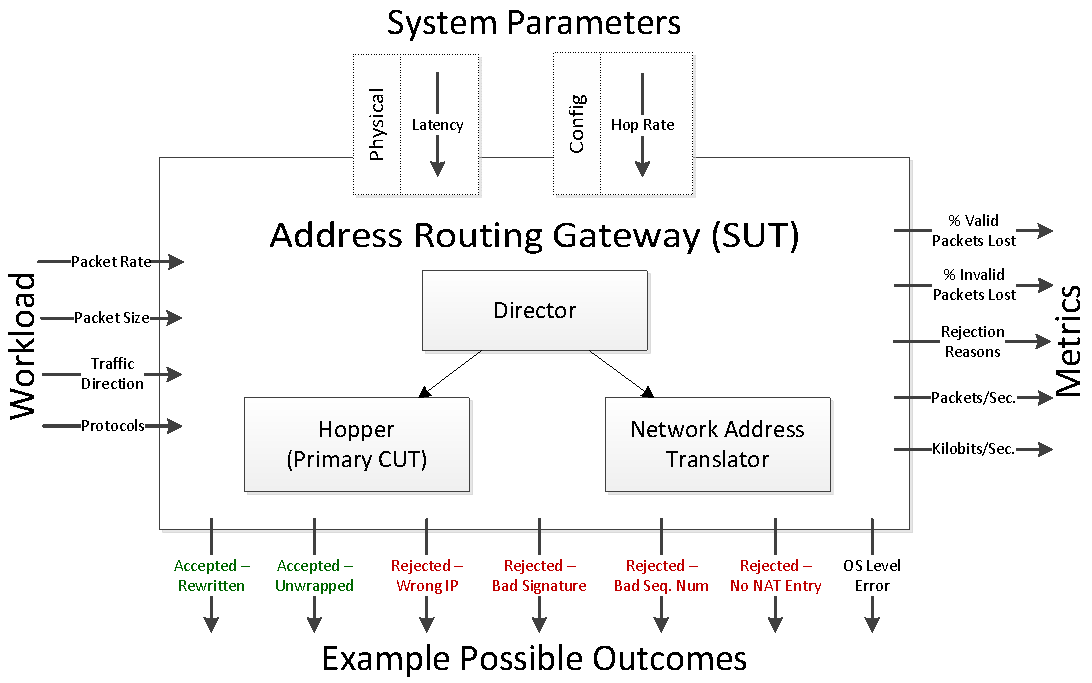
\includegraphics[width=1\textwidth]{../diagrams/sut}
	\caption{Address Routing Gateway}
	\label{fig:sut}
\end{figure}

\FloatBarrier
\section{System Services}
\label{sec:services}
\par The primary service provided by \ac{ARG} is the \ac{IPHC}. This service maintains a rapidly-changing external \ac{IP} address, details on paired \ac{ARG} networks, and other administrative information. Virtually all other aspects of \ac{ARG} rely on the information it provides. Most importantly, all packets leaving \ac{ARG} are altered to contain the current \ac{IP} as the source and, if the packet is destined for another paired \ac{ARG} network, the destination is changed to the current \ac{IP} for that gateway.

\par Rewriting \tbd{define what is meant by rewriting} is handled by the \ac{PTE}. Packets to and from non-\ac{ARG} networks (refered to ``extra-ARG'' \tbd{consider inter vs intra instead} traffic) are forwarded based on their source and destination identifiers (\acp{IP} and port numbers) via a lookup in a \ac{NAT} table. Packets to paired \ac{ARG} networks (referred to as ``inter-ARG'') are wrapped in \ac{IPv6} packets with header information from the \ac{IPHC} and extracted on the other end. Incoming packets that do not match the current gateway \ac{IP} or have an entry in the \ac{NAT} table---whichever is appropriate for the source of the packet---are rejected.

%\par Ultimately the simplest method of understanding \ac{ARG} is to view it as a router that p

\par Additionally, \ac{IPsec}-style encryption takes place between linked \ac{ARG} networks. This encryption may be disabled for speed, although previous research into \acp{DYNAT} found it to be an important factor in truly protecting the network \cite{BBNDYNAT, NAH}. Even without full encryption, \ac{ARG} still includes signatures for packets sent between \ac{ARG} networks for authentication and integrity. These signatures are used as a secondary rejection measure for packets claiming to be from a paired \ac{ARG} network. Packets to and from hosts outside a linked \ac{ARG} network are never encrypted or signed by the gateway (internal hosts may still use encryption for connections, just as on a normal network).

%\par Finally, \ac{ARG} provides a NAT table for connections to hosts outside paired \ac{ARG} networks. This table allows connections to persist across external \ac{IP} address changes and is vital for communications to outside hosts. Outgoing packets are transformed based on the data cached here and incoming packets are redirected to the correct internal host. Between \ac{ARG} networks, however, this table is not used. The maximum size of the table is configurable, from infinite (within memory and port number limits, obviously) to just a few on-going connections. This table is used as the primary rejection method for packets from non-\ac{ARG} networks. % TBD: use "linked" or "paired?"

\par The potential for the \ac{PTE} are shown below, broken into separate sections based on incoming or outgoing packets. Other services do not directly offer outcomes relevant to this research.
\begin{itemize}
\item \acl{PTE} - Incoming
	\begin{itemize}
	\item Rejected based on \ac{IP} - Packet is coming from an \ac{ARG} network but does not have the current local gateway \ac{IP} as the destination.
	\item Rejected based on signature - Packet signature invalid/nonexistent (if coming from an \ac{ARG} network).
	\item Rejected based on \ac{NAT} - Packet is coming from a non-\ac{ARG} network but does not have a valid entry in the \ac{NAT} table.
	\item Dropped - Processing queue full. If this outcome does occur the packet rate during experimentation will be slowed. Section \ref{sec:factors} provides more details.
	\item Unwrapped and forwarded - Packet is from \ac{ARG} network and passed the above tests. Contents are extracted and forwarded internally.
	\item Rewritten and forwarded - Packet is from non-\ac{ARG} network and is rewritten via \ac{NAT} table before forwarding.
	\end{itemize}
\item \acl{PTE} - Outgoing
	\begin{itemize}
	\item Wrapped and forwarded - Packet is destined for an \ac{ARG} network. Wrapped and placed on the external network.
	\item Rewritten and forwarded - Packet is destined for non-\ac{ARG} network. An entry is made/retrieved from the \ac{NAT} table and used to rewrite packet.
	\item Dropped - Processing queue is full.  If this outcome occurs the packet rate during experimentation will slow. Section \ref{sec:factors} provides more details.
	\end{itemize}
\end{itemize}

\section{Workload}
\label{sec:workload}
\par Workload to the system is the traffic flowing through the \ac{ARG} gateways. Standard network traffic parameters like packet rate, packet size, number of simultaneous ongoing connections, and lifetime of connections play a role. However, it is important to note that the network performance itself is not a large concern of this research. If \ac{ARG} begins dropping packets during experimentation, the network parameters and packet rate are reduced.

\par The only physical network parameter that has a major impact on \ac{ARG} is latency. To ensure that two \ac{ARG} gateways are able to communicate reliably, their hop rate must be less than two times the latency. If it is not, packets sent from one to the other will have the wrong \ac{IP} by the time they reach the destination. % TBD details on why... diagram showing traffic flow?

\par Two parameters are more specific to \ac{ARG}. First, the proportion of inter-\ac{ARG} verses extra-\ac{ARG} traffic varies the validation methods \ac{ARG} uses for each packet. Traffic flows that focus on inter-\ac{ARG} connections rely on current \ac{IP} synchronization and signatures, while traffic that originates externally exercises the \ac{NAT} table.

\par Second, the proportion of valid and invalid traffic---traffic that should or should not be permitted through \ac{ARG}---is a workload parameter. The reasons behind each packet's invalidity is also important: most of the possible outcomes from \ac{ARG} depend on \textit{why} a packet is invalid. The possible failure points here are incorrect external \acp{IP}, invalid packet signatures, and no entry in the \ac{NAT} table.

\section{Performance Metrics}
\label{sec:metrics}
\par As previously stated, this research is not particularly concerned with network performance directly. Details on this decision can be found in Section \ref{sec:boundaries}. Measurements on \ac{ARG} therefore focus on the outcomes from the \ac{PTE}. \tbd{Add stressing system to failure point to quantify performance bounds} These are:

\begin{itemize}
\item Proportion rejected/accepted packets to total transmitted
	\par With identical traffic flows, this provides a quick---albeit imperfect---check for changes in behavior between runs. This measurement cannot be relied upon for detailed analysis because it lacks any indication of why changes occur. For example, the system may reject based primarily on invalid signatures in one run and in a run with a faster hop rate reject primarily on incorrect IP, yet report similar rejection proportions.

\item Proportion of invalid packets accepted

	If a packet that should have been rejected is accepted by \ac{ARG}, it is possible for an attacker to sneak into the network regardless of the \ac{DYNAT}'s existence. This then is the true measure of whether or not \ac{ARG} is truly protecting the network. If it functions correctly, this number should remain at zero for all experiments with \ac{ARG} enabled.

\item Proportion of valid packets rejected
	\par In ideal circumstances, this will also be zero. However, network conditions may result in failures here, which on a real-world network might result in a disruption in service. It is also helpful to record bursts \tbd{how to record timing between failures} of failures, to discover why the system fails.

\item Number of each type of rejection (each possible outcome from the \ac{PTE})
	\par This reveals where in the processing stage packets are typically caught. If packets get caught in the later stages of validation---e.g., signature checking---then processing time has been wasted.
\end{itemize}

\section{System Parameters}
\par As a network application, \ac{ARG} is affected by standard network factors like bandwidth and latency. Additionally, the system each \ac{ARG} gateway runs on impacts its operation. The factors that come up most with \ac{ARG}'s local performance are memory speed and the processor speed and cores. As noted in Section \ref{sec:boundaries}, however, these aspects of the system are out of the scope of this research. 

\par \ac{ARG} also has several unique parameters that can be configured, allowing the actual \ac{SUT} to be tweaked. The primary configurable aspects of \ac{ARG} are:

\begin{itemize}
\item Hop rate
	\par \ac{ARG} allows the time between hops to be customized from several times a second to minutes apart. However, the hop rate is not fixed at that value; to compensate for latency spikes, \ac{ARG} may choose to slightly increase the hop rate (although it will always remain relatively close to the configured value).

\item Encryption
	\par Packets between \ac{ARG} gateways are always signed, but they can also be fully encrypted using symmetric keys. This operation can be disabled if desired for speed.

\item Threads
	\par \ac{ARG} runs several threads to process packets simultaneously, allowing it to more fully utilize the resources of the server on which it is running. The number of threads it uses is configurable.
\end{itemize}

\section{Factors}
\FloatBarrier
\label{sec:factors}
\par Based on the system and workload parameters given above, the following factors are varied as part of the experiment. All others remain constant throughout the experiment. Traffic proportions exclude administrative packets sent directly between \ac{ARG} gateways for synchronization. Factors and levels are summarized in Table \ref{tbl:factors} and described in detail below.

% A summary of the factors may be found in Table \ref{tab:factors}.

\begin{table}
\begin{center}
	\caption{Factors and Levels}
	\label{tbl:factors}
	
	\begin{tabular}{r|ccc}
		& Level 1 & Level 2 & Level 3 \\
	\hline
	Prop. inter-ARG vs. extra-ARG & 0.0 & 0.5 & 1.0 \\
	Prop. valid vs. invalid traffic & 0.0 & 0.5 & 1.0 \\
	Hop rate & None & Slow (\textasciitilde5 sec.) & Fast (< 1 sec.) \\
	Latency & Low (+5ms) & High (\textasciitilde+500ms) & Extreme (\textasciitilde+1000ms)
	\end{tabular}
\end{center}
\end{table}

\begin{itemize}
\item Proportion of inter-ARG verses extra-ARG packets
	\par Varying this parameter tests the extremes of traffic flow as well as a more typical situation with packets flowing many directions. It ensures that the system behaves correctly even if only one validation system \tbd{define earlier when talking about NAT and hopper} is ever put to use. The levels chosen for this study are listed below.

		\begin{itemize}
		\item 0.0 - All traffic is to systems outside \ac{ARG} networks.

		\item 0.5 - Half of the traffic on the network is to external hosts, half is to hosts in other \ac{ARG} networks. \tbd{add more levels here and the next one}

		\item 1.0 - All traffic is to hosts in other \ac{ARG} networks.
		\end{itemize}

	\par It is also be possible to add a fourth level with a proportion matching more real-world traffic flows. However, this will likely show no difference in behavior from 0.5.

\item Proportion of valid to invalid traffic
	\par This parameter hits at the heart of the research: just how good is \ac{ARG} (and \ac{IP} hopping in general) at detecting invalid traffic? The levels for this parameter are:
		\begin{itemize}
		\item 0.0 - All traffic sent to the \ac{ARG} gateways from external hosts is invalid.

		\item 0.5 - A simulation of the ``real world,'' where some traffic is valid---i.e., responses to traffic inside of \ac{ARG}---and some is not. 

		\item 1.0 - All traffic is valid. This level exists primarily to verify correct operation of \ac{ARG} and find cases where it incorrectly rejects packets.
		\end{itemize}

\item Hop rate
	\par Varying the rate at which \ac{ARG} switches to a new external \ac{IP} allows testing in circumstances where the rate of change may be low enough that an attacker can discover the current \ac{IP} and send packets through before the next switch. Additionally, it allows testing of the maximum supportable hop rate. The levels for this factor are:

		\begin{itemize}
		\item No hopping - Gateways do not actually hop at all during the test, an extreme case that separates synchronization issues from other factors of the system.

		\item Slow hopping (approximately 5 seconds per hop) - This length of time could allow an intruder to determine the current \ac{IP} and successfully have packets sent with the current data.

		\item Fast hopping (less than 1 second per hop) - Determining the current \ac{IP} and sending data before the gateway has moved to a new \ac{IP} is difficult for an attacker.
		\end{itemize}

\item Latency between \ac{ARG} gateways
	\par While there is an inevitable amount of latency in the experimentation, introducing additional artificial latency simulates an environment where the gateways are further apart. 

		\begin{itemize}
		\item Low (+20ms) - Latency is around a typical level for a \ac{WAN}, simulating relatively standard operating conditions.

		\item High (approximately +500ms) - Latency is significantly increased, likely affecting the ability of \ac{ARG} to communicate at fast hopping rates. Packets may occasionally arrive destined to the wrong \ac{IP}, even though they are otherwise valid, resulting in their rejection.
		
		\item Extreme (approximately +1000ms) - Latency is extremely high. The effects are similar to High latency, but greatly increased.
		\end{itemize}
\end{itemize}

\section{Evaluation Technique}
\label{sec:eval_technique}
\par Measurement is used to obtain results for each factor level. Due to the fairly complex interactions needed between \ac{ARG} gateways and the processing needed to decide how to handle packets, simulating the system in OPNET is infeasible. Even if possible, it would likely require equal work with little benefit.

\par Setup of the test environment involves a basic six-node network: two gateways running \ac{ARG}, one system on the network protected by each gateway, and two hosts outside the network. Figure \ref{fig:argnetwork} shows the network and the names given to the various systems.

\begin{figure}
	\centering
	\caption{ARG Network Layout Overview}
	\label{fig:argnetwork}
	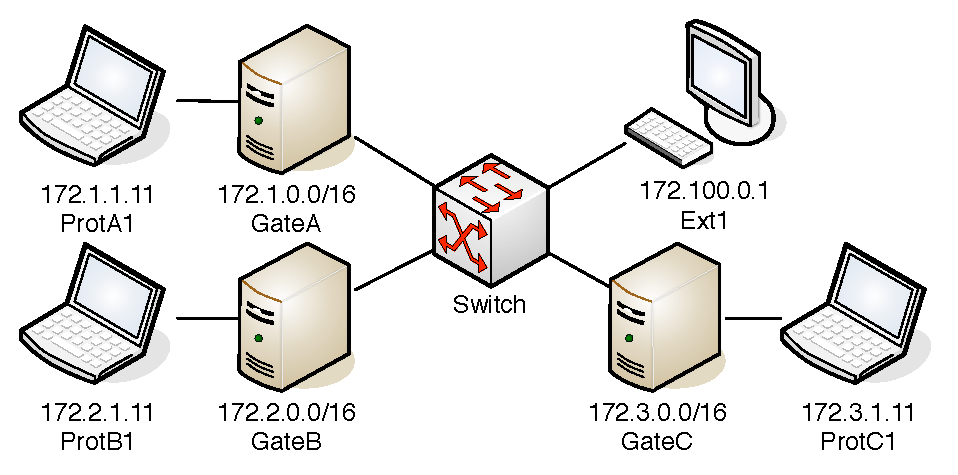
\includegraphics[width=0.75\textwidth]{../diagrams/thesis_network}
\end{figure}

\par Protected clients behind the gateways (\texttt{ProtA1} and \texttt{ProtB1}) may communicate freely. The protected clients may also talk out to the external hosts (\texttt{Extern1} and \texttt{Extern2}), and the external hosts must then---once that connection is established---be able to talk back into the network. These two basic traffic flows are ``valid'' traffic. There is additional administrative traffic directly between the gateways (\texttt{GateA} and \texttt{GateB}), but this is not relevant to the research itself \tbd{run pilot studies to prove this traffic has no effect}.

\par All traffic beyond what is described above is ``invalid.'' This traffic comes from \texttt{Extern1} and \texttt{Extern2} and is destined for either the protected clients or the gateways themselves. Invalid traffic may take several forms with varying levels of sophistication. At a basic level, an attacker may send in simple connection initiation attempts. More complex attacks by the external clients try to directly circumvent the validation methods used by the gateways: wrapping and fake-signing packet data, pretending to be the other gateway, piggybacking through via old \ac{NAT} table entries, and eavesdropping on the current gateway \acp{IP}.

\par To collect data, each system runs the traffic collection program \texttt{tcpdump} to capture the traffic sent and received. To make flows easier to identify, packets are tagged with a small amount of additional data. After a given trial runs, the traffic logs are collated and processed with custom scripts to determine the metrics described in Section \ref{sec:metrics}. The numbers generated here are then verified against counts that each system keeps on the number of valid and invalid packets they sent.

\par \tbd{implementation details on traffic generators and analyzers}

\par All trials run on a virtual network established within VMWare Workstation 8. The six systems described above run as \acp{VM} with Ubuntu 12.04 Server Edition.

\section{Experimental Design}
\label{sec:exp_design}
\par Based on the factors given in Section \ref{sec:factors}, a full factorial experimental design is feasible and allows the most complete analysis. The factors and levels listed in Section \ref{sec:factors} result in $3 \times 3 \times 3 \times 3 = 81$ unique experiments. Due to the possible impact of large network traffic disruptions, a 99\% confidence interval is used. Wide variation is possible in the actual traffic seen in a single run, so 10 replications are used for each experiment. This gives 810 total experiments.

\section{Methodology Summary}
\label{sec:method_summary}
\acresetall
\par This research determines if \ac{DYNAT}---the use of a gateway with a rapidly changing external \ac{IP} address---can effectively determine whether traffic should be allowed into a network. Several previous research efforts in this area already proved that \ac{DYNAT} made it more difficult to gain knowledge of a network \cite{BBNDYNAT} and that performance could be minimally impacted \cite{NAH}. 

\par A test network composed of two \ac{DYNAT}-protected networks and a few external hosts is used to explore this question. The custom \ac{DYNAT} solution used here, known as \ac{ARG}, allows the tuning of important system parameters. For the sake of this research, the primary factor is the hop rate. Levels used for experimentation include multiple times a second hops, several times a minute, and no hopping at all. Outside of \ac{ARG} itself, most hosts on the network run traffic generation scripts to simulate network activity. These scripts allow for the adjustment of packet rate, proportion of ``valid'' or ``invalid'' traffic produced, and how much traffic flows between the protected networks verses to the external hosts.

\par All hosts run the packet capture utilities, allowing custom analysis tools to run through each host's logs and pull out the desired metrics. For the research question posed above, the metrics include the overall rejection/acceptance rate of packets, incorrect classification of packets, and why packets are typically rejected. The factors and levels discussed in Section \ref{sec:factors} and the 10 replications result in 810 total experiments.

